\documentclass{IEEEcsmag}

\usepackage[colorlinks,urlcolor=blue,linkcolor=blue,citecolor=blue]{hyperref}
\expandafter\def\expandafter\UrlBreaks\expandafter{\UrlBreaks\do\/\do\*\do\-\do\~\do\'\do\"\do\-}
\usepackage{upmath,color}

\usepackage[spanish]{babel}
%\usepackage[latin1]{inputenc}
\usepackage[utf8]{inputenc}  

\jvol{1}
\jnum{1}
\paper{1}
\jmonth{Noviembre}
\jname{ITICs letters}
\jtitle{Proyectos Integradores}
\pubyear{2023}
\usepackage{cite}
\usepackage{amsmath,amssymb,amsfonts}
\usepackage{algorithmic}
\usepackage{graphicx}
\usepackage{textcomp}
\usepackage{xcolor}
\usepackage{listings}

\newtheorem{theorem}{Theorem}
\newtheorem{lemma}{Lemma}



\setcounter{secnumdepth}{0}

\begin{document}

%imprimir código
\lstnewenvironment{javaCode}[1][]
{\lstset{
    language=Java,
    basicstyle=\scriptsize\ttfamily,
    numbers=none, % Modificado: quitar los números de línea
    keywordstyle=\color{blue},
    commentstyle=\color{gray},
    stringstyle=\color{purple},
    breaklines=true,
    breakatwhitespace=true,
    tabsize=4,
    showspaces=false,
    showstringspaces=false,
    frame=single,
    captionpos=b,
    floatplacement=!h,
    #1
}}
{}


\sptitle{Proyecto Integrador de Primer Semestre}

\title{Software de resolución de problemas de Ingeniería }

\author{Daniel Aldana Lopez}
\affil{Instituto Tecnológico Superior del Occidente del Estado de Hidalgo, Actopan Hgo., 42500, México}

\author{Galilea Alonso Hernández}
\affil{Instituto Tecnológico Superior del Occidente del Estado de Hidalgo, Mixquiahuala, Hgo., 42700, Mexico}
\author{Carlos Granados Montoya}
\affil{Instituto Tecnológico Superior del Occidente del Estado de Hidalgo,  Francisco I Madero Hgo., 42675, México.}

\author{Ricardo López Cruz }
\affil{Instituto Tecnológico Superior del Occidente del Estado de Hidalgo, Mixquiahuala, Hgo., 42700, Mexico}
\author{Valeria Soto Hernandez}
\affil{Instituto Tecnológico Superior del Occidente del Estado de Hidalgo, Mixquiahuala, Hgo., 42700, Mexico}


%\author{Third Author III}
%\affil{Institute, City, (State), Postal Code, Country}

\markboth{ITSOEH/ITICS/PROYECTO INTEGRADOR PRIMER SEMESTRE}{THEME/FEATURE/DEPARTMENT}

\begin{abstract}
The integrative project is a didactic strategy that seeks that students apply, integrate and deepen the knowledge acquired in the different areas of the semester, through the resolution of a real and relevant problem. Students are organized in multidisciplinary teams and follow a process of research, design, implementation and presentation of an innovative solution to the problem posed based on the learning obtained during their school cycle in information technology and communications engineering. The primary objectives are to foster meaningful learning and the development of professional competencies, stimulate critical, creative and analytical thinking, promote collaborative work, effective communication and social responsibility, and generate new knowledge to be applied in real and diverse contexts. The integrative project has been an enriching and challenging learning experience for the students, who have achieved diverse learning and skills in problem solving, teamwork, communication, knowledge and professional competencies. \href{https://github.com/ricardoCruz2037/Proyecto-Integrador.git}{Puedes encontrar nuestro repositorio aquí}.
\end{abstract}
\maketitle
\chapteri{E}l objetivo del proyecto integrador es implementar el aprendizaje para abordar problemas matemáticos utilizando herramientas tecnológicas y software. Se busca mejorar la capacidad de razonamiento de los estudiantes de manera más eficiente y efectiva. Se espera que el estudiante pueda visualizar un modelo matemático preciso para representar el problema, seleccionar las herramientas adecuadas y utilizar una metodología que permita resolver los problemas planteados.

La metodología de las 6D es una técnica de resolución de problemas que se enfoca en 
\begin{itemize}
    \item Definir: En esta etapa, se establece claramente el problema o la situación a resolver. Se delimitan los objetivos, se identifican los problemas y se establecen los criterios para el éxito.
    \item Describir:Aquí se recopila información detallada sobre el problema. Se analizan las causas subyacentes, se investiga a fondo y se recopila la información relevante. 
    \item Diseñar:Se proponen soluciones posibles. En esta etapa se generan ideas y se elaboran diferentes enfoques para resolver el problema.
    \item Desarrollar:Se selecciona la mejor solución y se trabaja en su implementación. Aquí se crea un plan de acción detallado para llevar a cabo la solución elegida. 
    \item Depurar: Se implementa la solución y se prueba su eficacia. Se analizan los resultados y se comparan con los criterios establecidos en la etapa de definición.
    \item Documentación:Finalmente, se implementa la solución de manera más amplia si ha demostrado ser exitosa. Se lleva a cabo la difusión y se integra la solución en el contexto general.
\end{itemize}

Esta metodología proporciona una estructura sistemática para abordar problemas, facilitando la comprensión, la organización y la implementación de soluciones efectivas.

Dentro de este informe se tocaran 6 secciones:
\begin{itemize}
    \item La primera sección muestra la solución de un ejercicio que involucra la inserción de dos coordenadas para determinar la ecuación de una recta y el ángulo formado con el eje horizontal.

\item En la segunda sección, se aborda la solución de una ecuación cuadrática y se imprime el valor de sus raíces, siempre y cuando estén en el conjunto de números reales.
\item En la tercera sección, se encuentra la solución donde dada una circunferencia con centro en el punto C con coordenadas (x1 y1) y radio r, evaluar si un punto T con coordenadas (x2 y2) está dentro de la área de la circunferencia.
\item La cuarta sección, se aborda la solución donde dado un número decimal entero positivo o negativo regresar su equivalente en binario
\item La sección cinco presenta un código que permite ingresar un número binario de n bits y obtener su equivalente en número decimal.
\item Para terminar, en la sección seis se aborda la solución a una tabla de verdad  con una expresión booleana que genere de manera fidedigna las salidas de esta tabla
\end{itemize}

\section{COPYRIGHT Y ACCESO ABIERTO}

Una vez que los autores entreguen este documento para su evaluación también seden los derechos del contenido de este manuscrito a la carrera de Ingeniería en Tecnológicas de la Información y Comunicaciones (ITICs) del Instituto Tecnológico Superior del Occidente del Estado de Hidalgo (ITSOEH). Esto conlleva que la carrera puede usar el contenido de este articulo para efectos de difusión del quehacer de los estudiantes de la carrera o en cualquier otra actividad que la carrera considere pertinente. Cabe mencionar que en ningún momento el orden o los nombres de los autores sera modificado de ninguna manera y siempre se les dará el crédito correspondiente. 
\section{PROBLEMAS}
A continuación se describen los problemas que el equipo deberá resolver.
\begin{enumerate}
\item Dados 2 puntos $A \mbox{ y } B$ con coordenadas $x_{1}, y_{1}$ y $x_{2}, y_{2}$  respectivamente. Regresar la ecuación de la recta y el ángulo interno $\alpha$ que se forma entre el eje horizontal y la recta. 
%Por ejemplo con los puntos $A(2, 1)$ y $B(-3, 2)$ la ecuación debe ser $y = -\frac{1}{5}x + \frac{7}{5}$. 
\item Dada una ecuación cuadrática regresar los valores de las raíces en caso de que estén sobre el conjunto de los números reales, en caso contrario indicar que la solución esta en el conjunto de los números complejos. 
\item Dada una circunferencia con centro en el punto $C$ con coordenadas $(x_{1}, y_{1})$ y radio $r$, evaluar si un punto $T$ con coordenadas $(x_{2}, y_{2})$ esta dentro del área de la circunferencia.
\item Dado un numero decimal entero positivo o negativo regresar su equivalente en binario.
\item Dado un numero binario de $n$ bits regresar su equivalente en decimal.
\item Dada una tabla de verdad de $n$ bits generar la expresión booleana que genere de manera fidedigna las salidas de esta tabla.
\end{enumerate}
% PROBLEMA 1 -------------------------------------->Carlos
\section{Sección Problema 1: }
\section*{Descripción del problema:}Dados 2 puntos A y B con coordenadas x1, y1 y x2, y2 respectivamente. Regresar la ecuación de la recta y el ángulo interno que se forma entre el eje horizontal y la recta.

\section*{Definición de Solución} Primeramente debemos obtener nuestras coordenadas que son ingresadas por el usuario, para así poder calcular la pendiente, ecuación de la recta y ángulo interno.

\section*{Diseño de la Solución}{}
Para solucionar este problema debemos de seguir los siguientes pasos: 
\begin{itemize}
    \item Entrada de datos: 
El programa solicita al usuario que ingrese las coordenadas de dos puntos (A y B).
    \item Cálculo de la pendiente:
Utiliza la fórmula matemática de la pendiente para determinar el valor.
    \item Ecuación de la recta: 
Calcula la ecuación de la recta en la forma y = mx + c, donde 'm' es la pendiente y 'c' es el término independiente.
    \item Cálculo del ángulo: 
Determina el ángulo que la recta forma con el eje horizontal en radianes. 
    \item Convertir el ángulo de radianes a grados.
\end{itemize}
Tal y como se muestra en el siguiente diagrama de flujo.

\begin{figure}[h!]
    \centering
    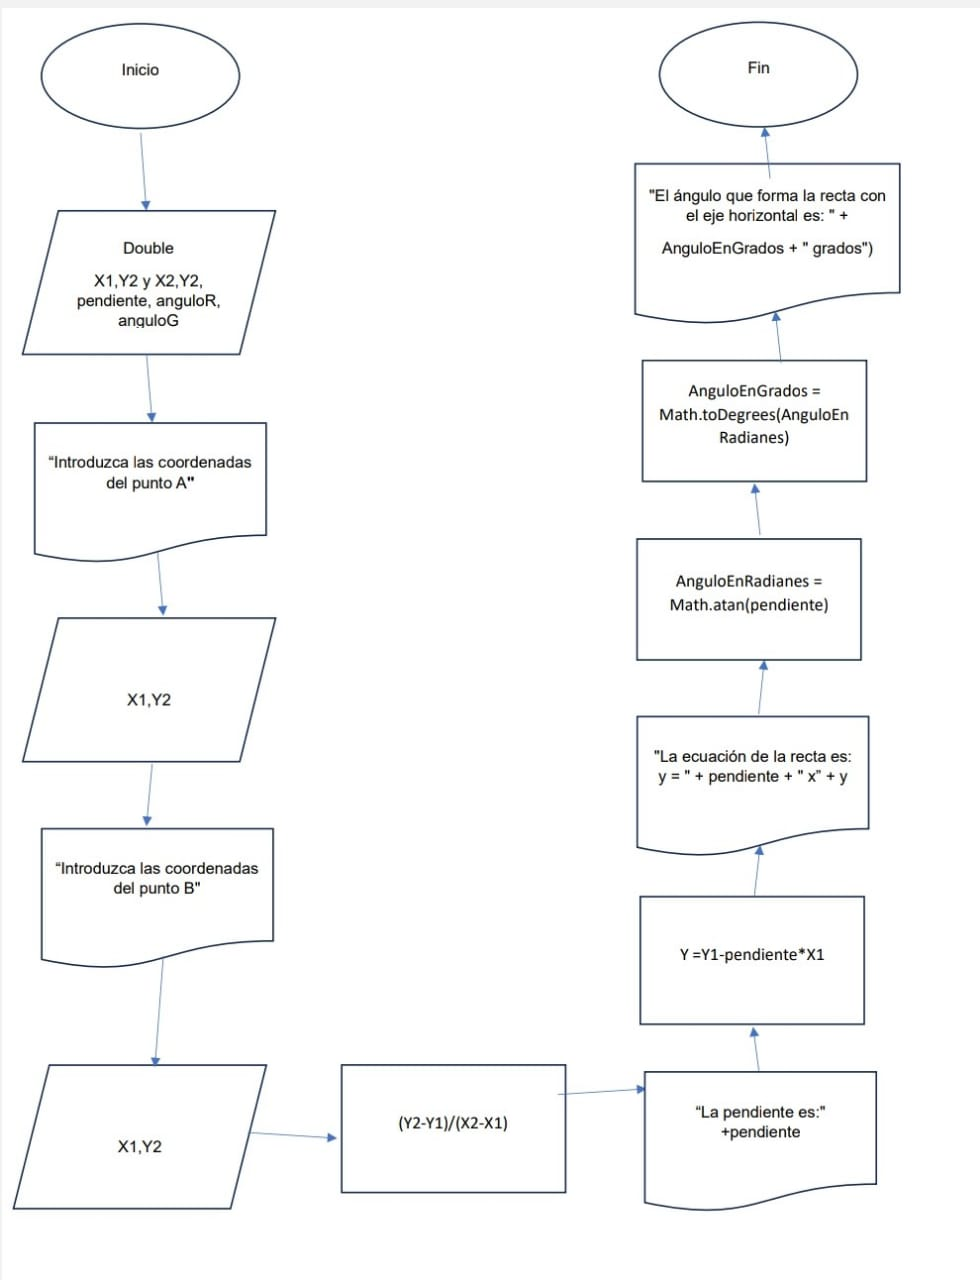
\includegraphics[width = 8 cm]{./latex-imagenes/DiagramaFlujo1.jpg}
    \caption{Diagrama de flujo del problema 1}
    \label{fig:Diagramadeflujode2 problema2}
\end{figure}

\section*{Desarrollo de la Solución}
Primeramente se definen las variables que vamos a utilizar como tipo double
\begin{javaCode}
  double x1,y1,x2,y2,pendiente,Y,
  AnguloEnRadianes,AnguloEnGrados
//Creamos nuestro objeto para poder leer datos 
Scanner c= new Scanner(System.in)
\end{javaCode}

Se le solicita al usuario ingresar las coordenadas del punto A y B
\begin{javaCode}
System.out.println("Introduzca las coordenadas del punto A ( x1 y y1 ) :");
//Se lee la entrada y se guardan en las variables correspondientes:
x1 = c.nextDouble();
y1 = c.nextDouble();
System.out.println("Introduzca las coordenadas del punto B ( x2 y y2 ) :");
//Se lee la entrada y se guardan en las variables correspondientes: 
x2 = c.nextDouble();
y2 = c.nextDouble();
\end{javaCode}
Se calcula la pendiente con las coordenadas ingresadas por el usuario y se acomoda de la forma de: 
\begin{javaCode}
y=mx+c
pendiente = (y2 - y1) / (x2 - x1);

//Se imprime el resultado de la pendiente

System.out.println("La pendiente es: " + pendiente);
\end{javaCode}
Se procede a calcular la ecuación de la recta en forma 
\begin{javaCode}
y = mx + c
Y = y1 - pendiente * x1;
//Se imprime la ecuacion de la recta 
System.out.println("La ecuacion de la recta es: y = " + pendiente + " x + " + Y);
\end{javaCode}
Con los resultados que ya tenemos procedemos a calcular nuestro ángulo, esto con funciones que ya vienen predeterminadas en nuestro lenguaje de java. 
\begin{javaCode}
AnguloEnRadianes = Math.atan(pendiente);

//Predeterminadamente nos da el angulo en radianes, por lo cual volvemos a utilizar funciones que ya estan programadas, para poder convertir de radianes a grados 

AnguloEnGrados = Math.toDegrees(AnguloEnRadianes);

//Imprimimos nuestros resultados, que son el angulo interno. 

System.out.println("El angulo que forma la recta con el eje horizontal es: " +
AnguloEnGrados + " grados");
\end{javaCode}
\section*{Depuración y pruebas:}

\begin{figure}[h!]
    \centering
    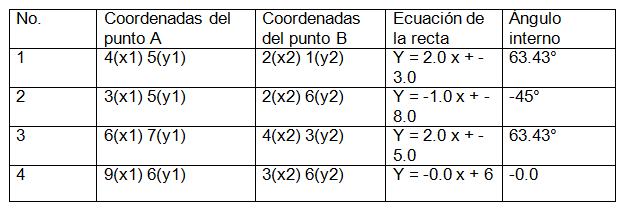
\includegraphics[width = 8 cm]{./latex-imagenes/TablaCorridas1.png}
    \caption{Tabla de pruebas Problema 1}
    \label{fig:Diagramadeflujode2 problema2}
\end{figure}
% PROBLEMA 2 ------------------------------------------>Vale
\section{Sección Problema 2} 
\section*{Descripción del problema:}
Se debe determinar si las raíces de una ecuación cuadrática son reales o complejas. Si son reales, se calculan y se proporcionan los valores. Si son complejas, se indica que la solución está en el conjunto de los números complejos.


\section*{Definición de solución:}
Para resolver el problema, primero debemos recordar que una ecuación cuadrática es de la forma:   (\(ax^2 + bx + c = 0\)) Donde a, b y c son números reales. Se obtiene y evalúa el discriminante, si es negativo, las raíces son complejas. De lo contrario, se calculan utilizando la fórmula cuadrática estándar:

\[ x = \frac{-b \pm \sqrt{b^2 - 4ac}}{2a} \]

Donde:
\begin{itemize}
    \item \(a\), \(b\), y \(c\) son los coeficientes de la ecuación cuadrática.
    
\end{itemize}
\begin{figure}[h!]
    \centering
    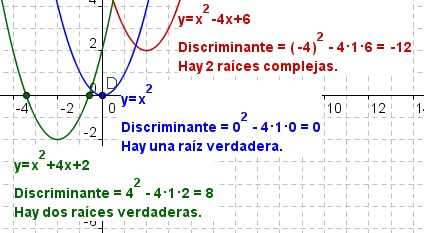
\includegraphics[width=0.6\linewidth]{./latex-imagenes/discriminant.png}
    \caption{Representación de los tipos de raíces}
    \label{fig: Grafica Ecuacion Recta}
\end{figure}
\section*{Diseño de la solución:}

Para el diseño de la solución se seguirán los siguientes pasos:
\begin{itemize}
    \item Definir las variables que van a ser utilizadas 
    \item Obtener los valores asignados a los coeficientes: a, b, c. 
    \item Calcular la discriminante
    \item Determinar si las raíces son reales o si son complejas 
    \item Si el discriminante es positivo, entonces las raíces son reales y distintas. En este caso, podemos utilizar la fórmula cuadrática para encontrar las raíces y devolverlas.
    \item Si el discriminante es cero, entonces las raíces son reales y coincidentes. En este caso, las dos raíces son iguales a -b/2a
    \item Si el discriminante es negativo, entonces las raíces son complejas. En este caso, la fórmula cuadrática no nos da una solución real. 
    \item El programa termina con la resolución de la problemática 
\end{itemize}

Tal y como se muestra en el siguiente diagrama de flujo.

\begin{figure}[h!]
    \centering
    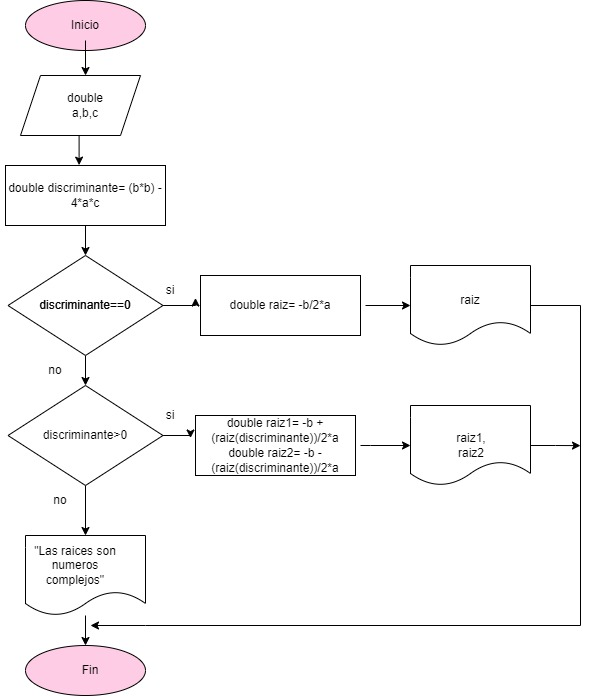
\includegraphics[width = 8 cm]{./latex-imagenes/DiagramaFlujo2.jpg}
    \caption{Diagrama de flujo del problema 2}
    \label{fig:Diagramadeflujode2 problema2}
\end{figure}

\section*{Desarrollo de la solución:}
Definir desde un inicio todas las variables que se van a usar dentro del programa
\begin{javaCode}
// Declarar las variables
        double a,b,c, raiz1, raiz2, discrminante;
\end{javaCode}
Como se menciono con anterioridad, se le solicita al usuario ingresar el valor de los coeficientes \(a\), \(b\), y \(c\), siendo posible que ingrese números reales 
\begin{javaCode}
Scanner dato=new Scanner(System.in);
        //Obtener datos
        System.out.println("Ingresa los coeficientes de la ecuacion cuadratica");
        System.out.print("a: ");
        a=dato.nextDouble();
        System.out.print("b: ");
        b=dato.nextDouble();
        System.out.print("c: ");
        c=dato.nextDouble();
\end{javaCode}
Para definir si nuestra raíz se encuentra en el conjunto de los números reales o está en el conjunto de los complejos se hace uso del valor del discriminante, el siguiente paso a realizar es calcular su valor con los datos ya obtenidos
\begin{javaCode}
//Calcular el discriminante
        discrminante=Math.pow(b, 2)- 4*a*c;
\end{javaCode}
Ya que tenemos el resultado de la discriminante, dependiendo de este se realizara la operación justa, o se dirá que la discriminante esta dentro de los números complejos.
En caso de que la discriminante sea igual a cero, las dos raíces son iguales a -b/2a y se imprime el resultado en pantalla.
\begin{javaCode}
    if(discrminante==0){
          double  raiz=-b/(2*a);
            System.out.println("La ecuacion tiene una raiz real: ");
            System.out.println("Raiz: "+raiz);
        }
\end{javaCode}
Si el discriminante es positivo, es decir, mayor que cero, entonces las raíces son reales y distintas. En este caso, podemos utilizar la fórmula cuadrática para encontrar las raíces y devolverlas. Se imprimen en pantalla los 2 posibles resultados:
\begin{javaCode}
    else if(discrminante >0){
            raiz1=(-b + Math.sqrt(discrminante))/(2*a);
            raiz2=(-b - Math.sqrt(discrminante))/(2*a);
            System.out.println("La ecuacion tiene dos raices reales: ");
            System.out.println("Raiz 1: "+raiz1);
            System.out.println("Raiz 2: "+raiz2);
        }
\end{javaCode}
Por ultimo, si el discriminante es negativo, entonces las raíces son complejas. En este caso, la fórmula cuadrática no nos da una solución real. 
\begin{javaCode}
  else{
            System.out.println("Las raices son numeros complejos");
        } 
\end{javaCode}

\section*{Depuración y pruebas:}
\begin{table}[h]
     \centering
     \begin{tabular}{|c|c|c|c|c|}
\hline
\textbf{\(No.\)} & \textbf{\(a\)} & \textbf{\(b\)} & \textbf{\(c\)} & \textbf{\(Resultado\)} \\
\hline
1 & 4 & 8 & -12 & Raíces reales: \(x_1 = 1, x_2 = -3\) \\
\hline
2 & 1 & -3 & 2 & Raíces reales: \(x_1 = 2, x_2 = 1\) \\
\hline
3 & 4 & 12 & 9 & Raíz real única: \(x = -3/2\) \\
\hline
4 & 2 & 4 & 8 & Raíces complejas \\
\hline
\end{tabular}
     \label{tab:my_label}
     \caption{Tabla de pruebas Problema 2}
 \end{table}

%  PROBLEMA 3 ------------------------------------------>Daniel
\section{Sección Problema 3} 
\section*{Descripción del problema:}
Dada una circunferencia con centro en el punto C con coordenadas (x1, y1) y radio r, evaluar si un punto T con coordenadas (x2, y2) está dentro del área de la circunferencia.

\section*{Definición de solución:}
Teniendo como referencia que para validar que un punto T está dentro de la circunferencia inicial con punto C y radio R. Se busca validar si la distancia entre el punto T y C es mayor o menor o igual al radio R.  Puesto que si es mayor, el punto T no estará dentro de la circunferencia, y de lo contrario, este punto estará dentro. 
Para evaluar la distancia entre dos puntos utilizamos la ecuación: 
\newline
\newline

\begin{figure}[h!]
    \centering
    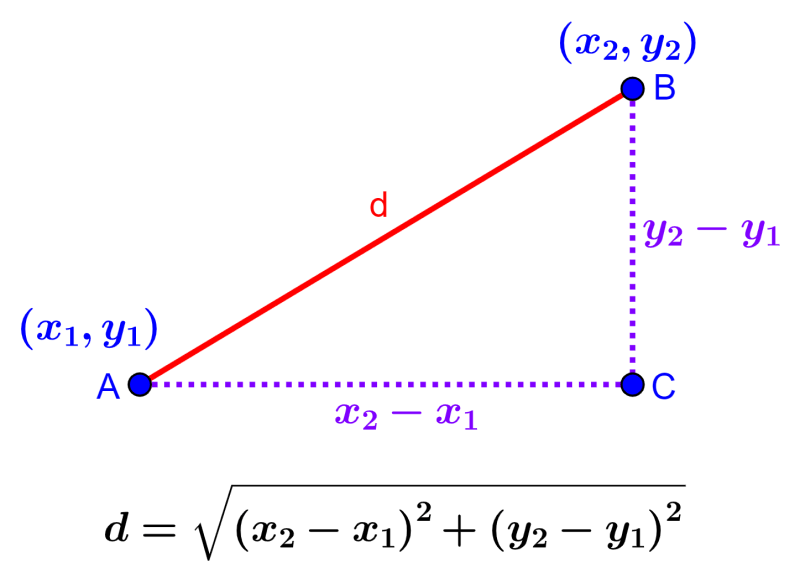
\includegraphics[width=0.6\linewidth]{./latex-imagenes/Ecuacion.png}
    \caption{Representación de la ecuación de distancia}
    \label{fig: Grafica Ecuacion Recta}
\end{figure}

\section*{Diseño de la solución:}
\setlength{\parskip}{5pt}
Para el diseño de la solución se utilizó el siguiente razonamiento:
\begin{enumerate}
    \item La fórmula de la distancia entre dos puntos en un plano se basa en el teorema de Pitágoras. Supongamos que tenemos dos puntos C(x1,y1) y T(x2,y2) en un sistema de coordenadas cartesianas. La distancia d entre estos dos puntos se puede encontrar usando el teorema de Pitágoras en un triángulo rectángulo formado por los dos puntos y el punto en el origen con coordenadas (0,0).\newline
    \newline
    El teorema de Pitágoras establece que en un triángulo rectángulo, el cuadrado de la hipotenusa (c) es igual a la suma de los cuadrados de los catetos (a y b). En el contexto de la distancia entre dos puntos, podemos expresar esto de la siguiente manera:
    \begin{equation}
        c^2 = a^2 + b^2
    \end{equation}

    En nuestro caso, C es la distancia entre los puntos C y T(d), a es la diferencia en las coordenadas x menos x2 menos x1, y b es la diferencia en las coordenadas y y2 menos y1.

    Definir variables:\newline
    X1, x2, y1, y2, R, Distancia: Serán valores de tipo Double\newline
    El punto de las coordenadas (x1,y1) representará el punto C\newline
    El punto de las coordenadas (x1,y1) representará el punto T\newline
    La distancia será definida por la ecuación: \newline
    La condición que define si el punto T está dentro de la circunferencia es: \newline
    Si Distancia <= R el punto T está dentro de la circunferencia \newline

    Tal y como se muestra en el siguiente diagrama de flujo.

    \begin{figure}[h!]
        \centering
        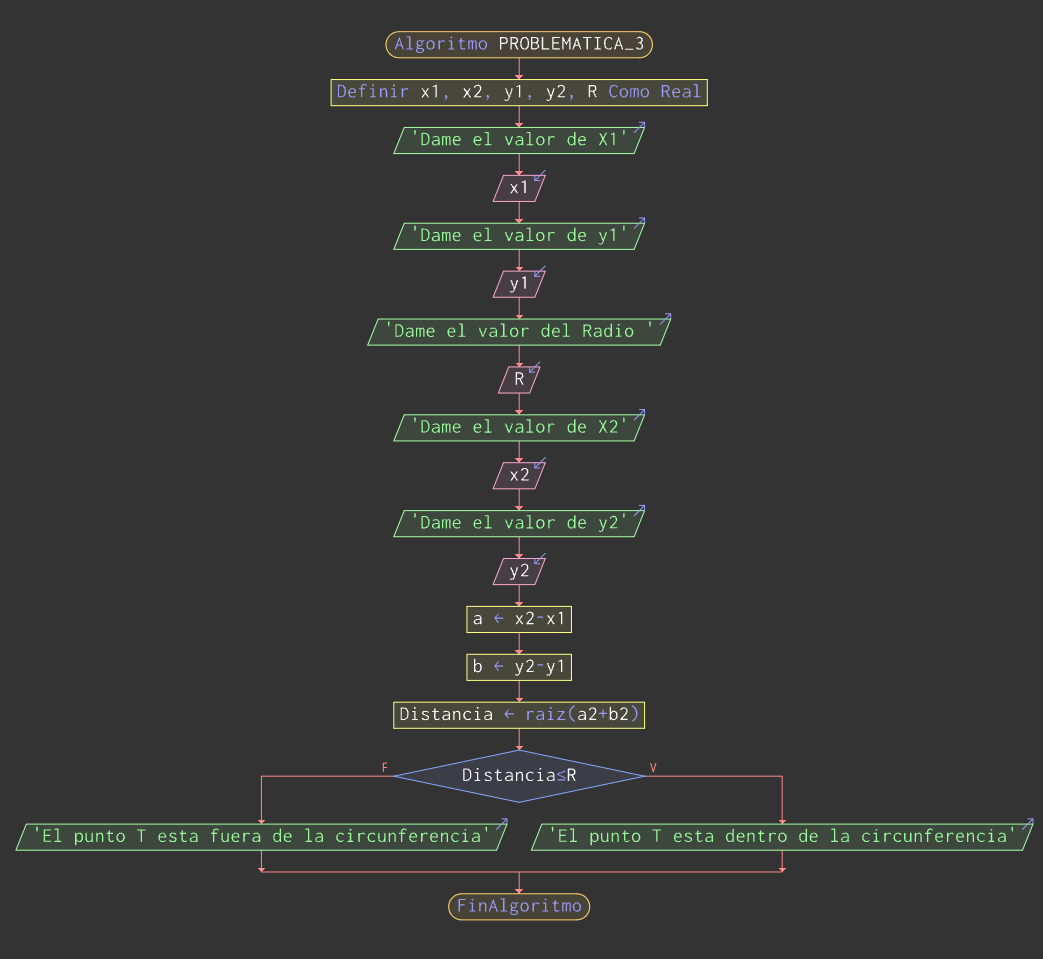
\includegraphics[width=8 cm]{./latex-imagenes/Diagrama.png}
        \caption{Diagrama de flujo del problema 3}
        \label{fig:Diagramadeflujode2 problema2}
    \end{figure}
\end{enumerate}

\section*{Desarrollo de la solución:}
\setlength{\parskip}{5pt}
\begin{enumerate} 

\item Solicitar al usuario las coordenadas del centro de la circunferencia. El usuario ingresa la coordenada X1,Y1 correspondiente al punto C.\newline
\begin{javaCode}
// Solicitar al usuario las coordenadas del centro de la circunferencia
System.out.print("Ingrese la coordenada x1 del centro de la circunferencia: ");
double x1 = scanner.nextDouble();

System.out.print("Ingrese la coordenada y1 del centro de la circunferencia: ");
double y1 = scanner.nextDouble();
\end{javaCode}


\item El usuario ingresa el valor del radio R.
\begin{javaCode}
// Solicitar al usuario el radio de la circunferencia
System.out.print("Ingrese el radio de la circunferencia: ");
double r = scanner.nextDouble();
\end{javaCode}




\item Solicitar al usuario las coordenadas del punto a verificar. El usuario ingresa la coordenada X2,Y2 correspondiente al punto T.
\begin{javaCode}
// Solicitar al usuario las coordenadas del punto a verificar
System.out.print("Ingrese la coordenada x del punto a verificar: ");
double x2 = scanner.nextDouble();

System.out.print("Ingrese la coordenada y del punto a verificar: ");
double y2 = scanner.nextDouble();
\end{javaCode}



\item Calcular la distancia entre el centro de la circunferencia y el punto dado.
\begin{javaCode}
// Calcular la distancia entre el centro de la circunferencia y el punto dado
double distancia = Math.pow((x2 - x1), 2) + Math.pow((y2 - y1), 2);
\end{javaCode}



\item Verificar si el punto está dentro de la circunferencia
\begin{javaCode}
// Verificar si el punto esta dentro de la circunferencia
if (distancia <= r) {
    System.out.println("El punto esta dentro de la circunferencia.");
} else {
    System.out.println("El punto esta fuera de la circunferencia.");
}
\end{javaCode}

\end{enumerate}
\section*{Depuración y pruebas:}
\begin{table}[h]
     \centering
     \begin{tabular}{|c|c|c|c|c|c|c|}
\hline
\textbf{\(No.\)} & \textbf{$X_1$ } & \textbf{$Y_1$ } & \textbf{$R$ }& \textbf{$X_2$ } & \textbf{$Y_2$ } & \textbf{\(Resultado\)} \\
\hline
1 & -5 & -48 & 85 & 4 & 4 & Fuera \\
        \hline
        2 & 3 & 4 & 5 & 1 & 2 & Fuera \\
        \hline
        3 & 1 & 2 & 5 & 3 & 4 & Dentro \\
        \hline
        4 & -1 & -1 & 2 & -1 & 0 & Dentro \\
\hline
\end{tabular}
     \label{tab:my_label}
     \caption{Tabla de pruebas Problema 3}
 \end{table}

%  PROBLEMA 4------------------------------------------>Ricardo
\section{Sección Problema 4}
\section*{Descripción del problema:}
Dado un número decimal entero (ya sea positivo o negativo), realizar las operaciones necesarias para obtener su equivalencia en el sistema binario. En caso de que sea negativo, hacer uso del método de bit de signo (también conocido como complemento A2).


\section*{Definición de la solución:}
La conversión de números enteros a binario se puede dividir en dos partes: la conversión de números enteros positivos y la conversión de números enteros negativos.

Conversión de números enteros positivos

El método más utilizado para convertir un número entero positivo a binario es el método de Leibniz. Este método consiste en dividir el número decimal por 2 repetidamente, tomando el resto de cada división como un bit del número binario resultante.

\section*{Diseño de la solución:}

Para resolver el problema de la conversión de números decimales a binarios, se debe seguir los siguientes pasos:

Identificar el funcionamiento de la conversión de números decimales a binarios
El primer paso es entender cómo funciona la conversión de números decimales a binarios. Esta conversión se basa en la representación de los números decimales en base 2. Por lo tanto, cada bit de un número binario representa una potencia de 2.
 \begin{itemize}
\item Determinar el alcance del código.
El segundo paso es determinar el alcance del código. En este caso, se busca que el código funcione hasta 64 bits y que sea capaz de leer tanto números positivos como negativos.

\item Diseñar el proceso de conversión para números positivos.
El tercer paso es diseñar el proceso de conversión para números positivos. Este proceso se basa en dividir el número decimal por 2 repetidamente, tomando el resto de cada división como un bit del número binario resultante.


\item 4/2 = 2 --> residuo 0
\item 2/2 = 1 --> residuo 0
\item 1/2 = 0 --> residuo 1
 \end{itemize}
 
Para representar un número negativo en binario, se obtiene la representación binario del numero ingresado por el usuario, luego, obtenemos el valor absoluto del número Binario. Una vez que tenemos el valor absoluto, invertimos sus bits, comenzando por el primer bit 1 que encontremos, de derecha a izquierda.

Guardaremos la posición donde se encuentre el primer número 1, luego, a este se le sumara 1 para avanzar a la siguiente posición sin que la original guardada no se vea afectada. Es ahí cuando realizamos nuestra siguiente operación para invertir el bit almacenado en dichas posiciones siguientes del primer 1.

\begin{itemize}
\item numeroBinario[i] = 1 - numeroBinario[i];
\item Valor de la posición = 1 - Valor de la posición.
\item Si el Valor de la posición es 0: 1 - 0 = 1. Por lo que tenemos ahora como valor 1.
\item Si el Valor de la posición es 1: 1 - 1 = 0. Por lo que tenemos ahora como valor 0. 
\end{itemize}

De esta forma tendremos invertido nuestros bits y habremos realizado el complemento A2 de nuestro número negativo, cumpliendo así con la problemática principal del problema y cumpliendo con el objetivo principal de la conversión correcta del número decimal a binario.

Una vez ya diseñamos la logística detrás de nuestro algoritmo, se realizo el diagrama de flujo en el que se mostrara como va a ser el funcionamiento de este y como podríamos codificarlo. En el se pueden apreciar distintas funciones las cuales detallaré en el desarrollo.

\begin{figure}[h!]
    \centering
    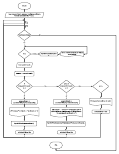
\includegraphics[width=0.6\linewidth]{./latex-imagenes/DiagramaFlujo4.png}
    \caption{Representación del funcionamiento del algoritmo.}
    \label{fig: Diagrama de flujo.}
\end{figure}

\section*{Desarrollo de la solución:}

En el desarrollo de la solución del problema 4, se diseñaron nuevas funciones para evitar el uso de funciones preestablecidas de Java. La función imprimirBinario recorre el arreglo que almacena el número binario, imprimiendo el valor de cada posición.

\begin{javaCode}
	private static void imprimirBinario(long[] numeroBinario) {
		for (int j = numeroBinario.length - 1; j >= 0; j--) {
			System.out.print(numeroBinario[j]);
		}
	}
\end{javaCode}

numeroBinario: La función numeroBinario genera el número binario del número ingresado por el usuario. Para ello, realiza un bucle que divide el número por 2 repetidamente. El residuo de cada división se almacena en un arreglo. El número binario se obtiene leyendo los valores del arreglo de atrás hacia adelante.

\begin{javaCode}
	private static long[] conversionBinario(long numeroUsuario) {
		long[] numeroBinario = new long[64];
		int i = 0;

		while (numeroUsuario != 0) {
			long division = numeroUsuario / 2;
			long modulo = numeroUsuario % 2;
			numeroBinario[i] = modulo;
			numeroUsuario = division;
			i++;
		}

		return numeroBinario;
	}
\end{javaCode}

calcularComplementoDos: Por último, La función calcularComplementoDos se encarga de calcular el complemento a dos de un número binario. El complemento a dos de un número es el número que, sumado al número original, da como resultado 1.
La función calcularComplementoDos funciona de la siguiente manera:
\begin{itemize}
\item Invierte los bits del número binario, a partir de la primera posición con valor 1.
\item Realiza la operación de resta, donde a un número 1 se le estará restando el valor de la posición actual.
Por ejemplo, para calcular el complemento a dos del número binario 1011, se realizarían los siguientes pasos:
\item Se encuentra la primera posición con valor 1, que es la segunda posición.
\item Se invierten los bits siguientes a esa posición, es decir, el tercer y cuarto bit.
\item Se realiza la operación de resta, donde a un número 1 se le está restando el valor de la posición actual.

El resultado de la operación es el número binario 0100, que es el complemento a dos de 1011.
\end{itemize}

\begin{javaCode}
	private static long[] calcularComplementoDos(long[] numeroBinario) {
		// Encuentra el primer 1 en la representacion binaria
		int primerUno = -1;
		for (int i = 0; i < numeroBinario.length; i++) { // Recorre el array hasta a la posicion del primer 1, partiendo
															// de
			// esta, comienza a invertir los bits.
			if (numeroBinario[i] == 1) {
				primerUno = i;
				break;
			}
		}

		// Invierte los bits desde el primer 1
		for (int i = primerUno + 1; i < numeroBinario.length; i++) {
			numeroBinario[i] = 1 - numeroBinario[i]; // Si binario es 0 = 1-0=1. por lo que tenemos ahora binario de 1.
		} // Si binario es 1 = 1-1=0. por lo que tenemos ahora binario de 0.

		return numeroBinario;
	}
\end{javaCode}
\section*{Depuración y pruebas:}
Una forma sencilla de verificar el correcto funcionamiento del algoritmo es utilizar un número conocido. En este caso, se puede utilizar el número 4, que se sabe que su representación binaria en 64bits es 00000000 00000000 00000000 00000000 00000000 00000000 00000000 00000100. Si el algoritmo devuelve este número, entonces funciona correctamente.

Utilizar un número que tenga una representación binaria de 64 bits. En este caso, se puede utilizar el número 9223372036854775807, que se sabe que su representación binaria es 01111111 11111111 11111111 11111111 11111111 11111111 11111111 11111111. Si el algoritmo devuelve este número, entonces funciona correctamente.

\begin{figure}[h!]
    \centering
    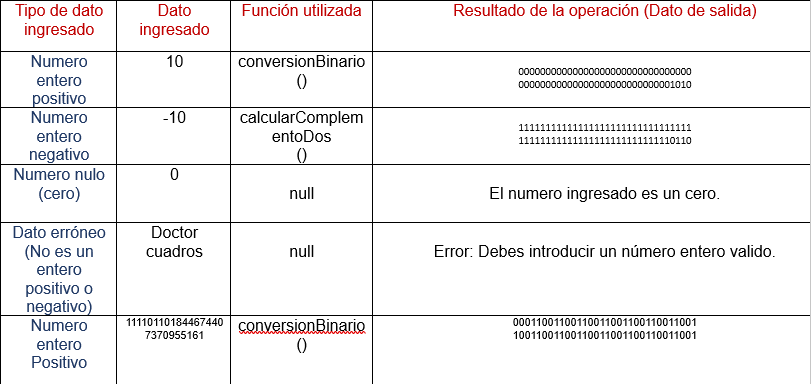
\includegraphics[width=1.0\linewidth\centering]{./latex-imagenes/tablaDePruebas.png}
 
    \caption{Como podemos observar, se depura nuestro código de distintas maneras, tales que podemos ver el  funcionamiento de este para cada caso, ya sea que el numero ingresado sea positivo, negativo, 0, o que se ingrese otro tipo de dato no correspondiente.}
    \label{fig: Depuraciones.}
\end{figure}

% PROBLEMA 5 ------------------------------------------>Galilea
\section{Sección Problema 5}

\section*{Descripción del problema:  }
Dado un numero binario de n bits regresar su equivalente en decimal

\section*{Definición de la solución:} 
Primero debemos identificar n bits que es nuestro numero binario a ingresar y se le asigna la potencia de 2 colocándose de derecha izquierda, una vez sacada la potencia de cada bit se multiplica cada dígito por correspondiente potencia de 2 y se suman los términos obtenidos lo que equivale el numero binario a decimal 


\section*{Diseño de la solución:}

Para la solución de el problema se llevara a cabo los siguientes pasos:

\begin{itemize}
	\item Definir las variables dependiendo lo que se pide  
	\item Asignar el valor correspondiente (base-2)
	\item Se le incrementa el exponente a uno de derecha a izquierda 
	\item Sacar la potencia con nuestra variable definida (Math.pow)
	\item Se multiplican los dígitos obtenidos por el numero binario
	\item Se suman los términos 
	\item El programa imprime los resultados 
\end{itemize}

    Diagrama de flujo:  
\begin{figure}[h!]
    \centering
    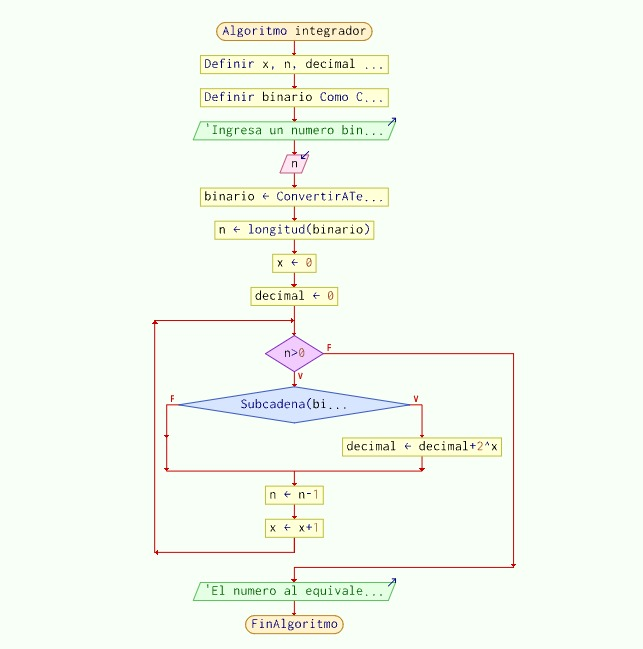
\includegraphics[width = 8 cm]{./latex-imagenes/DiagramaFlujo5.jpg}
    \caption{Diagrama de flujo del problema 5}
    \label{fig:Diagramadeflujode2 problema2}
\end{figure}
  
\section*{Desarrollo de la solución:}
Definir la clase y las variables a utilizar
\begin{javaCode}
Binario, potencia, decimal 
\end{javaCode}
Se crea el objeto para leer la entrada del usuario
\begin{javaCode}
	Scanner s = new Scanner(System.in);
\end{javaCode}
Se le solicita al usuario ingresar el numero de n bits (Numero binario) 
\begin{javaCode}
	System.out.print("Ingresa un numero binario: ");
\end{javaCode}
La entrada se lee como una cadena y se guarda en una variable de tipo String
\begin{javaCode}
	String binarioString = s.nextLine();
\end{javaCode}
Se declara las variables de tipo long para obtener un rango de valores mas amplio
\begin{javaCode}
	int longt = binarioString.length();
\end{javaCode}
La variable decimal se declara de tipo int para almacenar el valor decimal equivalente al numero binario
\begin{javaCode}	
	int decimal = 0;
\end{javaCode}
Se declara de tipo int para hacer la conversión de binario a decimal 
\begin{javaCode}
	int potencia = 0;
\end{javaCode}
Se inicia un ciclo for que inicializa la variable i con el valor de longt - 1 (la longitud del número binario menos 1). El ciclo se ejecuta mientras i sea mayor o igual a 0, y en cada iteración, i se decrementa.

El int digito devuelve el carácter en la posición i de la cadena binarioString. La resta '0' convierte el carácter a su valor numérico.

La conversión y acumulación donde se multiplica el dígito (digito) por 2 elevado a la potencia actual (Math.pow(2, potencia)) y se suma al acumulador decimal. La variable potencia se incrementa después de cada repetición para manejar la posición del dígito en el número binario.
 \begin{javaCode}
for (int i = longt - 1; i >= 0; i--) {
	int digito = binarioString.charAt(i) - '0';
	decimal += digito * Math.pow(2, potencia);
	potencia++;
}
\end{javaCode}
Por ultimo se hace la impresión del programa 
\begin{javaCode}
 System.out.println("El numero binario " + binarioString + " en decimal es: " + decimal);
\end{javaCode}
\section*{Depuración y pruebas:}
\begin{table}[h]
     \centering
     \begin{tabular}{|c|c|c|}
     \hline
        No. & Binario & Decimal\\
        \hline
        1  & 110 & 6\\
        \hline
        2  & 10000000000 & 1024\\
        \hline
        3  & 110010 & 50\\
        \hline
        4  & 11001 & 25\\
        \hline
     \end{tabular}
     \label{tab:my_label}
     \caption{Tabla de pruebas Problema 5}
 \end{table}
% PROBLEMA 6------------------------------------------>Vale
\section{Sección Problema 6}
\section*{Descripción del problema:}
Dada una tabla de verdad de 2 a 5 bits generar la expresión booleana que genere de manera fidedigna las salidas de esta tabla.
\section*{Definición de solución:}
El problema consiste en generar una expresión booleana a partir de una tabla de verdad de 2 a 5 bits. La tabla de verdad contiene todas las combinaciones posibles de valores de entrada. El usuario debe definir cuantas salidas de esta tabla desea que sean verdaderas y posteriormente cuales son. El programa finaliza cuando imprime la expresión booleana

\section*{Diseño de la solución:}
El diseño se basa en tres funciones principales:
\begin{enumerate}
\item Leer el número de bits (numB) del usuario.
\item Calcular el número de combinaciones posibles (combinaciones) = 2 elevado al numB
\item Imprimir el encabezado de la tabla según el número de bits.
\item Imprimir un separador.
\item Imprimir todas las combinaciones posibles de bits.
\item Leer la cantidad de salidas deseadas (salidasC) del usuario.
\item Leer las salidas deseadas (salidas) del usuario.
\item Imprimir las expresiones booleanas que representan las salidas deseadas por el usuario.
\end{enumerate}

\section*{Desarrollo de la solución:}
Obtener por parte del usuario el numero de bits con los que se va a generar e imprimir la tabla así como el numero de combinaciones posibles. Se debe de imprimir un encabezado diferente de acuerdo a la cantidad de bits
\begin{javaCode}
Scanner d=new Scanner(System.in);
        System.out.println("Ingresa la cantidad de bits");
        int numB=d.nextInt();
        
        int combinaciones=(int) Math.pow(2, numB);
        //Imprimir encabezado de la tabla de acuerdo al numero de bits 
            switch (numB) {
                case 2:
                    System.out.print(" A "+"\t"+" B "+"\t");
                    break;
                case 3:
                    System.out.print(" A "+"\t"+" B "+"\t"+" C "+"\t");
                    break;
                case 4:
                    System.out.print(" A "+"\t"+" B "+"\t"+" C "+"\t"+" D "+"\t");
                    break;
                case 5:
                    System.out.print(" A "+"\t"+" B "+"\t"+" C "+"\t"+" D "+"\t"+" E "+"\t");
                    break;      
            }
        System.out.println("No. Salida");
        
        //Imprimir separador
        for(int i=0; i< numB + 1;i++){
        System.out.print("---------");
        }
        System.out.println();
        //Combinacion de bits posibles
        for(int i=0;i< combinaciones ;i++){
        for(int j=0;j< numB;j++){
        int bit=(i>>j)&1;
        System.out.print(bit+"\t");   
        }
        System.out.println(i);
        }
\end{javaCode}
Obtener por parte del usuario el numero de salidas que desea sean verdaderas (1) así como su No. de combinación, esta información será almacenada en un arreglo llamado salidas[]
\begin{javaCode}
System.out.println("Teclea la cantidad de salidas que deseas sean verdaderas(1)");
        int salidasC=d.nextInt();
        int [] salidas=new int [salidasC];
        for(int i=0;i< salidasC;i++){
        System.out.println("Teclea el numero de salida que deseas sea verdadera(1)");
        salidas[i]=d.nextInt();
        }
\end{javaCode}
\newpage
Genera la expresión booleana a partir de las salidas que se seleccionaron como verdaderas. 
\begin{javaCode}
System.out.println("La expresion es: ");
        switch(numB){
            case 2:{
           for(int i=0;i<salidasC;i++){
               if(salidas[i]==0){
                   System.out.print("A' B'");
               }
               if(salidas[i]==1){
                   System.out.print("A B'");
               }
               if(salidas[i]==2){
                   System.out.print("A' B");
               }
               if(salidas[i]==3){
                   System.out.print("A B");
               }
               if(i+1<salidasC){
                   System.out.print(" + ");
               }
            }
            System.out.println();
            }
            break;
            
            case 3:{
           for(int i=0;i<salidasC;i++){
               // Codigo con las posibles salidas, 8 posibles salidas
            }System.out.println();}
            break;
            
            case 4:{
           for(int i=0;i<salidasC;i++){
           // Codigo con las posibles salidas, 16 posibles salidas
            }System.out.println();}
            break;
            
            case 5:{
           for(int i=0;i<salidasC;i++){
               // Codigo con las posibles salidas, 32 posibles salidas
               }
            } System.out.println();}
        
\end{javaCode}

\section*{Depuración y pruebas:}

\begin{table}[h]
\centering
\begin{tabular}{|c|c|c|c|c|}
\hline
\textbf{Nº} & \textbf{A} & \textbf{B} & \textbf{C} & \textbf{Salida} \\
\hline
0 & 0 & 0 & 0 & 0 \\
1 & 1 & 0 & 0 & 1 \\
2 & 0 & 1 & 0 & 0 \\
3 & 1 & 1 & 0 & 0 \\
4 & 0 & 0 & 1 & 0 \\
5 & 1 & 0 & 1 & 0 \\
6 & 0 & 1 & 1 & 1 \\
7 & 1 & 1 & 1 & 0 \\

\hline
\end{tabular}
\caption{Tabla de pruebas Problema 6}
\end{table}
Expresión booleana: $AB'C' + A'BC$
\section{CONCLUSIÓN}

Conclusión

El presente proyecto ha demostrado la eficacia de la metodología 6D para el desarrollo de software para la resolución de problemas de ingeniería. Los resultados obtenidos son un claro ejemplo de la versatilidad de esta metodología, que permite integrar conceptos de diversas disciplinas matemáticas para generar soluciones prácticas y claras.

Más allá de la creación del software, este proyecto ha destacado la importancia del proceso de resolución de problemas mediante la programación.

Este proyecto abre nuevas posibilidades para futuras investigaciones en la intersección de la programación y las matemáticas, así como para la aplicación de la metodología 6D en otros contextos de la ingeniería.
\vspace*{-8pt}


\section{AGRADECIMIENTOS}
Agradecemos a la docente Eunice Santiago manzano y al Dr. Francisco Javier Cuadros romero quienes se encargaron de asesorar al equipo en las dudas y en apoyar con información valiosa para la modificación del proyecto

\begin{IEEEbiography}{Daniel Aldana Lopez}{\,}
Daniel es un joven entusiasta de 18 años amante de la tecnología y con aspiraciones por la misma. Actualmente su objetivo principal es ser mejor cada día, y se encuentra estudiando le primer semestre de ingeniería en TIC´S. Sueña con ser millonario y hacer del mundo un lugar mejor.Su pagina personal se encuentra disponible en \href{https://dani-ald.github.io/}{https://dani-ald.github.io/}.
\end{IEEEbiography}
\begin{IEEEbiography}{Galilea Alonso Hernández}{\,}Es un estudiante de ITICs que tuvo en interés en conocer mas afondo sobre la carrera y conocer bien las herramientas de software para solventar desafíos a lo largo de la carrera. Espera aprender a programar lo mejor que pueda para llevar a cabo su profesión en un futuro en el mundo laboral, una de las cosas que más le gusta hacer es bailar y escuchar canciones norteñas mientras hace su tarea.Su pagina personal se encuentra disponible en \href{https://github.com/fcuadrosgithub/integrador-primero.git}{https://github.com/fcuadrosgithub/integrador-primero.git}.
\end{IEEEbiography}
\begin{IEEEbiography}{Carlos Granados Montoya }{\,}Es actualmente un estudiante de la carrera de TICS en el Instituto Tecnológico Occidental del Estado de Hidalgo (itsoeh) desde pequeño se interesó demasiado por la tecnología y por las cosas que se pueden crear con estas herramientas, la principal razón por la cual ingresó a este Instituto es para poder ayudar a muchas personas a resolver problemas y hacer la vida más fácil, tiene un gran interés por el hacking ético, porque parece algo muy interesante en este mundo.
\end{IEEEbiography}
\begin{IEEEbiography}{Ricardo López Cruz }{\,} Es un estudiante de ITICs que tiene una relación un tanto contradictoria con la tecnología. Este interés le impulsó a estudiar dicha carrera, ya que desde adolescente le ha fascinado la idea de dominar temas que en un principio podrían no parecer fáciles de comprender. Actualmente, su objetivo es más que pasar las materias con un 100, es dominar y comprender los temas que le resulten útiles a la hora de aplicarlos a la vida laboral, además de crear vínculos que lo lleven por caminos relacionados con la carrera. Uno de sus sueños es crear una empresa de inversiones junto con sus más grandes camaradas, con quienes comparte su pasión por la tecnología y el humor. Su pagina  personal se encuentra disponible en \href{https://ricardocruz2037.github.io/.github.com/}{https://ricardocruz2037.github.io/.github.com/}.\end{IEEEbiography}
\begin{IEEEbiography}{Valeria Soto Hernández}{\,}Estudiante de ITICs. Su objetivo principal  es completar sus estudios universitarios en ITICs, ya que sueña con trabajar en el campo del desarrollo de software, nada impresionante, solo busca una vida tranquila con un buen salario. Su pagina  personal se encuentra disponible en \href{https://valeriasot0.github.io/}{https://valeriasot0.github.io/}.
\end{IEEEbiography}

\end{document}




\end{document}